\chapter{Lambda Calculus}

\pagenumbering{arabic}
The Lambda Calculus is an example of a formal system which consists a language of lambda terms and some auxiliary notions such as \textit{free variables} and \textit{subterms}, and the transformation theory. The core of the theory is the notion of substitution - the driving force behind function application. 


\section{$\lambda$-terms}

\noindent The expressions in lambda calculus can be formalized into following: 


\begin{def1}
\normalfont \textbf{($\lambda$-TERMS)} $\lambda$-terms can be defined by the following rules:
\end{def1}

\begin{itemize}
\item a variable, $x$, itself is a lambda term
\item if $M$ is a lambda term, and $x$ is a variable, then $(\lambda x.M)$ is a lambda term
\item if $M$ and $N$ are both lambda terms, then \textit{(MN)} is a lambda term
\end{itemize}
A lambda term is valid if and only if it can be obtained by repeated application of these rules. However, some parentheses can be omitted in certain forms. For example the leftmost, outer-most brackets are usually omitted.

\textbf{A lambda abstraction $\lambda x.M$} takes a single input x and returns a term M. Thus, it defines an \textbf{anonymous} function. For example $\lambda x.x^2$ is a lambda abstraction for the function $f(x) = x^2$ using the term $x^2$ for M, then we can say that $f = \lambda x.x^2$. The function is anonymous since we write $(x^2)2$ rather than $f3$.

\textbf{An application $(MN)$} applies the input term N to the function M. For example $(\lambda x.x^2)2$ is an application that applies 2 to the function $f(x) = x^2$, it return $2^2$ which equals 4.

As mentioned above, leftmost, outer-most brackets are usually omitted. Therefore, $M_1M_2(M_3M_4)$ stands for $((M_1\cdot M_2)(M_3\cdot M_4))$. Similarly, $\lambda$ can be omitted in repeated abstractions, for example $\lambda x_1x_2.M$ stands for $\lambda x_1.(\lambda x_2.M)$.

\begin{def1}
\normalfont \textbf{(free and bound variables)} The set of free and bound variables are defined inductively by the following function:
\end{def1}

\begin{equation*}\label{eq:fv}
\begin{array}{lcllcl}
FV(x)           & = & \{x\}             & BV(x)           &=& \emptyset\\
FV(\lambda x.M) & = & FV(M)\backslash \{x\} & BV(\lambda x.M) &=& BV(M)\cup \{x\}\\
FV(MN)          & = & FV(M)\cup FV(N) & BV(MN)          &=& BV(M)\cup BV(N)
\end{array}
\end{equation*}


For example, the lambda term $\lambda x.x$ has no free variables but a bound variable $x$. The function $\lambda x.x+y$ only has a single free variable $y$ and a bound variable $x$. 
Notice that, the sets of bound and free variables are not necessarily disjoint; $x$ occurs both bound and free in:
\begin{equation*}
x(\lambda xy.x)
\end{equation*}


\section{Substitution}

\noindent A cursory approach to define the substitution operation leads to the problem of \textit{variable capture}. It occurs when we substitute a term containing a free variable into a scope where the variable becomes bound. For example:
\begin{equation*}
(\lambda xy.xy)y \neq \lambda y.yy
\end{equation*} 

The free occurrence of y in the left hand term becomes confused with the bound variable after substitution.To avoid \textit{variable capture}, we define a capture-avoiding substitution. The notion $[x:=N]$ indicates the replacement of a variable $x$ by a term $N$:

\begin{equation*}
\begin{array}{lrll}
(1)&x[x:=N]&=N & ~\\
(2)&y[x:=N]&=y,& if\ y\neq x\\
(3)&(\lambda y.M)[x:=N]&=\lambda y.M,& if\ y=x\\
(4)&(\lambda y.M)[x:=N]&=\lambda y.(M[x:=N]),& if\ y\notin FV(N)\ \& \ y\neq x\\
(5)&(\lambda y.M)[x:=N]&=\lambda z.(M[y:=z])[x:=N],& if\ y\in FV(N)\ \& \ y\neq x,z\  new\\
(6)&(M_1M_2)[x:=N] &= (M_1[x:=N])(M_2[x:=N])&
\end{array}
\end{equation*}

\begin{def1}\label{def1}
\normalfont \textbf{($\alpha$-equivalent)} \textit{$M$ is $\alpha$-equivalent to $N$, written $M$ $\equiv_\alpha N$, if $N$ results from $M$ by a series of changes of bound variable.}
\end{def1}

The notion of alpha-equivalent(or congruence) is a basic form of equivalence defined in lambda calculus. It captures the property that the particular choice of a bound variable in a lambda abstraction does not matter. For instance, $\lambda x.x$ and $\lambda y.y$ are $\alpha$-congruent lambda terms which represent the same function. Notice that, the term-variable $x$ and $y$ are not $\alpha$-equivalent terms since they are not bound in a lambda abstraction.

With the property of alpha equivalence, we can define the \textit{$\alpha$-conversion}:

\begin{equation*}
\lambda x.M =_\alpha \lambda z.(M[z:=x])
\end{equation*}

In some sense, the $\alpha$-conversion is defined by the spirit of the (5) substitution rule. If we have a function $\lambda x.M$, then we can apply a substitution to this function: $(\lambda x.M)[z:=x]$. According to the fifth substitution rule, it is unfolded to $(\lambda z.M[z:=x])$. Using the $\alpha$-conversion, we can always rename the bound variables of a term. 

\begin{def1}
\normalfont \textbf{(Variable Convention \cite{hankin1994lambda})} \textit{In a $\lambda$-term, all bound variables are chosen to be different from free variables.}
\end{def1}

The alpha-conversion is built based on the variable convention. Alpha conversion is used to allow bound variable names to be changed. For example, alpha-conversion of $\lambda x.x$ might get $\lambda y.y$. Terms that differ only by alpha-conversion are called alpha-equivalence(or alpha-congruence) as mentioned in the definition \ref{def1}. By the assumption that free and bound variables are always different(variable convention), and that alpha-conversion will take place whenever a variable is both free and bound. The definition of term substitution becomes:
\begin{equation*}
\begin{array}{rll}
x[x:=N]&=N & ~\\
y[x:=N]&=y,& if\ y\neq x\\
(\lambda y.M)[x:=N]&=\lambda y.(M[x:=N])& \\
(M_1M_2)[x:=N] &= (M_1[x:=N])(M_2[x:=N])&
\end{array} 
\end{equation*}

By this definition of term substitution, the \textit{variable capture} is avoided. Since that y is bound in $\lambda y.M$ of the context:
\begin{equation*}
\lambda y.M[x:=N]
\end{equation*}
$y$ can only be bound in $N$ according to variable convention rule, otherwise, if $y$ is also free in $N$, it would be renamed by another variable. 

Here is an example of its use:
\begin{equation*}
\begin{array}{ll}
&(\lambda xy.xy)(\lambda xy.xy)\\
\Rightarrow& \lambda y.(\lambda xy.xy)y \\
\Rightarrow & \lambda yz.yz\ \ \mathrm{by\ the\ alpha \ convension} \\
\end{array}
\end{equation*}

\section{$\beta$-reduction}

\noindent There are various notions of reduction for $\lambda$-terms, but the principle one is $\beta$-reduction. $\beta$-reduction is the one-step reduction relation, written as $'\rightarrow _\beta'$. 

\begin{def1}
($\beta$-reduction) For $\lambda$-terms $M$ and $N$, we say that $M$ $\beta$-reduces in one step to $N$, written as $M \rightarrow _\beta N$:
\end{def1}
\begin{equation*}
(\lambda x.M)N\rightarrow _\beta M[x:=N]
\end{equation*}

\begin{equation*}
\frac{M\rightarrow _\beta N}{MZ \rightarrow _\beta NZ}
\end{equation*}
\begin{equation*}
\frac{M\rightarrow _\beta N}{ZM \rightarrow _\beta ZM}
\end{equation*}
\begin{equation*}
\frac{M\rightarrow _\beta N}{\lambda x.M \rightarrow _\beta \lambda x.N}
\end{equation*}

\noindent The reduction relation, written $'\twoheadrightarrow _\beta'$, is the reflexive, transitive closure of the one-step reduction relation. The one-step reduction relation allows a single step of reduction, while the reduction relation allows many steps. The reflexive transitive closure is defined as follows:
\begin{equation*}
\frac{M\rightarrow _\beta N}{M \twoheadrightarrow _\beta N}
\end{equation*}
\begin{equation*}
M \twoheadrightarrow _\beta M
\end{equation*}
\begin{equation*}
\frac{M\twoheadrightarrow _\beta N\ \ \ \ N\twoheadrightarrow _\beta Z}{M \twoheadrightarrow _\beta Z}
\end{equation*}

For the notion $'M\rightarrow _\beta N'$, it is read as '$M$ $\beta$-reduces to $N$'. The first rule defines that the reduction relation is reflexive to one-step reduction relation, while the third rule indicates the transitivity of reduction relation.

\noindent Finally, the $\beta$-equality, written as '$=_\beta$'. For $\lambda$-terms $A$ and $B$, we say that $A =_\beta B$ if either $A \equiv B$ or there exists a sequence of reduction starting with $A$, ending with $B$. It is the equivalence relation generated by $\twoheadrightarrow _\beta$:

\begin{equation*}
\frac{M\twoheadrightarrow _\beta N}{M = _\beta N}
\end{equation*}
\begin{equation*}
\frac{M = _\beta N}{N = _\beta M}
\end{equation*}
\begin{equation*}
\frac{M = _\beta N\ \ \ \ N = _\beta Z}{M = _\beta Z}
\end{equation*}

For the notion $'M = _\beta N'$, we say '$M$ $\beta$-equivalent to $N$'. 

\noindent Following is a simple example which applies $\beta$-reduction:

\begin{equation*}
\begin{array}{ll}
&(\lambda abc.ac(bc))(\lambda xy.x)\\
\Rightarrow& \lambda bc.(\lambda xy.x)c(bc) \\
\Rightarrow& \lambda bc.(\lambda y.c)(bc)\\
\Rightarrow& \lambda bc.c \\
\end{array}
\end{equation*}


\begin{def1}
($\beta$-redex) A $\beta$-redex of a $\lambda$-term $M$ is a subterm of M of the form ($\lambda$x.P)Q. A term M is called in $\beta$-normal form if it has no $\beta$-redex.
\end{def1}
A $\beta$-redex is essentially a candidate for an application of $\beta$-reduction. A term $M$ has a $\beta$-normal form if there exists a term N such that N is in $\beta$-normal form and $M \twoheadrightarrow _\beta N$. 

\section{Head Normal Form}

\noindent A $\lambda$-term in head normal form is generally in the form:

\begin{equation*}
\lambda x_1\ldots x_n.xM_1\ldots M_m\ \ \ \ \ \ \ \ n,m\geqslant 0
\end{equation*}

In this case $x$ is called the head variable. If $M \equiv \lambda x_1\ldots x_n.(\lambda x.M_0)M_1\ldots M_m$ where $n\geqslant 0$, $m\geqslant 1$ then the subterm $(\lambda x.M_0)M_1$ is called the head redex of $M$. Following are some examples of $\lambda$-terms in head normal form:
\begin{equation*}
(1)\ xM\ \ \ \ (2)\ \lambda x.x\ \ \ \ (3)\ \lambda xy.x((\lambda z.z)y)
\end{equation*}Normal order:
Notice that, an expression in head normal form may contain redexes in argument positions whereas a normal form may not.


\section{Reduction strategies}\label{sec:reductionstrategy}
\noindent Recall that a term is said to be in $\beta$-normal form if it has no $\beta$-redexes, that is, subterms of the shape ($\lambda$x.M)N. A term has a $\beta$-normal form if it can be reduced to a term in $\beta$ in $\beta$-normal form. It is clear that if a term has a $\beta$-normal form, then we can get to the $\beta$-normal form by exhaustively reducing all $\beta$-redexes of the term, then reducing all $\beta$-redexes of all resulting terms, and so forth until we get the $\beta$-normal form. A \textbf{$\beta$-reduction strategy} is a function that selects, whenever a term has multiple $\beta$-redexes, which one should be reduced first. If a term is in $\beta$-normal form, then no $\beta$-reduction is to be done. Notice that, a $\beta$-reduction strategy may or may not have the property that adhering to the strategy will ensure that we(eventually) can normalize a $\lambda$-term. 

In general, there are several different $\beta$-reductions possible for a given term. In this project, there are 5 different reduction strategies studied and implemented: normal order, call-by-name, call-by-value, head reduction, and applicative order. Table \ref{tb:rd} generally summarizes and compares the property of different strategies:
 
\begin{table}[h]
\begin{tabular}{|l|l|l|l|}
\hline
Reduction Strategy & Reduction Order                                                                                            & Reach $\beta$-normal form & Form Reached          \\ \hline
Normal Order       & leftmost outer-most                                                                                         & Yes                       & normal form           \\ \hline
Call-by-Name       & \begin{tabular}[c]{@{}l@{}}leftmost outer-most\\ not inside an abstraction\end{tabular}                     & No                        & weak head normal form \\ \hline
Call-by-Value      & \begin{tabular}[c]{@{}l@{}}leftmost inner-most \\ not inside an abstraction\end{tabular}                    & No                        & weak normal form      \\ \hline
Head Reduction     & \begin{tabular}[c]{@{}l@{}}reduction inside lambda\\ abstractions but only in\\ head position\end{tabular} & No                        & head normal form      \\ \hline
Applicative Order  & leftmost inner-most                                                                                         & Yes                       & normal form           \\ \hline
\end{tabular}
\caption{Property of different reduction strategies}
\label{tb:rd}
\end{table}

It would be introduced in Chapter \ref{chap:haskell}, lambda terms are modelled as Haskell constructed data, representing variable names by character:

\begin{verbatim}
             type Name = Char  

             data Term = Var Name | Abs Name Term | App Term Term
                         deriving (Show, Eq)
\end{verbatim}


\subsection*{Operational Semantics}

Operational semantics are a category of formal programming language semantics in which certain desired properties of a program, such as correctness, safety or security, are verified by constructing proofs from logical statements about its execution and procedures, rather than by attaching mathematical meanings to its terms (denotational semantics) \cite{operational}. The final step of a terminating sequence returns the resulting value of the program. Operational semantics can be classified into two types: \textbf{structural operational semantics(SOS or small-step semantics)} and \textbf{natural semantics(NS or big-step semantics)}. The structural operational semantics describes each single step of a computation in a program, while the natural semantics describes the overall resulting value generated by the program. Following, we use both SOS and NS to define the behaviour of each reduction strategy. The small-step semantics gives reduction rules of the strategy, when the big-step semantics describes how the final term is reached.  

\subsection*{Recursion}

Although a reduction strategy may or may not have the property that ensures it reaches a $\beta$-normal form, it would recursively contract the selected redex until no redex(decided by specific reduction strategy) can be contracted. All the following Haskell functions defined corresponding to the reduction strategy model the small-step semantics. Therefore, in order to recursively reduce a $\lambda$-term, an auxiliary function \verb|recur_eval :: Term -> IO()| is defined:

\begin{verbatim}
       recur_eval :: Term -> IO()
       recur_eval t | evalcbn t == t = putStrLn("")
                    | otherwise = do
                                putStrLn("==> "++ tostring (evalcbn t))
                                recur_eval (evalcbn t)
\end{verbatim}

The Haskell function above defines the recursive reduction using Call-by-Name strategy. It uses the small-step function defined in Section \ref{subsec:cbn}. It uses `guards' to list two cases: 1. The recursion will terminate if the input $\lambda$-term cannot be reduced further. 2. Otherwise, it would print-out the term after a single step reduction and continue reducing the resulting term.



\subsection{Call-by-Name Reduction}{\label{subsec:cbn}}

The Call-by-Name reduction reduces the leftmost outer-most redex not insde a lambda abstraction first. That is, the arguments to a function are not evaluated before the function is called. The redex in $e$ of the asbtraction $(\lambda x.e)$ will never be reduced. 


\begin{equation*}
\llceil x \rrfloor ^{ls} _{cbn} = x
\end{equation*}
\begin{equation*}
\llceil (\lambda x.e) \rrfloor ^{ls} _{cbn} = (\lambda x.e)
\end{equation*}
\begin{equation*}
\frac{\llceil e_1 \rrfloor ^{ls} _{cbn} = (\lambda x.e)\ \ \ \ \ \ \ \ \ \llceil e[e_2/x] \rrfloor ^{ls} _{cbn} = e'}{\llceil (e_1e_2) \rrfloor ^{ls} _{cbn} = e'}
\end{equation*}
\begin{equation*}
\frac{\llceil e_1 \rrfloor ^{ls} _{cbn} = e'_1\neq (\lambda x.e)}{\llceil (e_1e_2) \rrfloor ^{ls} _{cbn} = (e'_1e_2)}
\end{equation*}
\begin{center}
Call-by-Name: Big-step operational semantics
\end{center}

\begin{equation*}
\frac{}{(\lambda x.M)N \rightarrow _\beta M[N/x]}\ \ \ \  
\frac{M \rightarrow _\beta N}{MP \rightarrow _\beta NP}\ \ 
\end{equation*}
\begin{center}
Call-by-Name: Small-step operational semantics
\end{center}

The Call-by-Name reduction generates term in weak head normal form. A lambda expression is in weak head normal form if it is a head normal form or any lambda abstraction. 


The corresponding Haskell function \verb|evalcbn :: Term -> Term| below implements the Call-by-Name reduction:

\begin{verbatim}
       --call-by-name reduction
       evalcbn :: Term -> Term
       evalcbn (Var x) = Var x
       evalcbn (Abs x t) = (Abs x t)
       evalcbn (App (Abs x t) y) = subs t (Var x, y)
       evalcbn (App x y) | x == evalcbn x = (App x y)
	                     | otherwise = (App (evalcbn x) y) 
\end{verbatim}


The first two function clauses handle the variables and abstractions, it returns itself since they cannot be reduced under Call-by-Name reduction. The third function implements the first SOS rule which performs substitution. The last function implements the second SOS rule: the argument of an application will not be reduced before the function is called. 

\begin{exmp}
\normalfont The same example in \ref{subsec:normal} run in Haskell by the Call-by-Name strategy is as follows:
\end{exmp}


\begin{verbatim}
           (/a.a)(/b.b)((/x.x)(/y.(/z.z)w))
       ==> (/b.b)((/x.x)(/y.(/z.z)w))
       ==> (/x.x)(/y.(/z.z)w)
       ==> /y.(/z.z)w
       Reduced to:/y.(/z.z)w
\end{verbatim}

It is easy to see that the first three reduction steps are the same as normal order reduction. In this example, it stops at $\lambda y.(\lambda z.z)w$. Since the difference between normal order and call-by-name is the redex inside abstractions will never be reduced in call-by-name, and the argument will not be reduced before the function is called. 

\subsection{Normal Order Reduction}{\label{subsec:normal}}

The normal order reduction continually applies rules for $\beta$-reduction on the redex in leftmost outer-most position until no more $\beta$-reduction can be performed. At that point, the resulting term is in normal form. When reducing an application $(e_1e_2)$, the function term $e_1$ must be reduced using call-by-name. Since the strategy is outer-most, when $e_1$ is reduced to an abstraction $(\lambda x.e)$, then the redex $((\lambda x.e)e_2)$ must be reduced before redexes in e.

\begin{equation*}
\llceil x \rrfloor ^{ls} _{no} = x
\end{equation*}
\begin{equation*}
\frac{\llceil e \rrfloor ^{ls} _{no} = e'}{\llceil (\lambda x.e) \rrfloor ^{ls} _{no} = (\lambda x.e')}
\end{equation*}
\begin{equation*}
\frac{\llceil e_1 \rrfloor ^{ls} _{cbn} = (\lambda x.e)\ \ \ \ \ \ \ \ \ \llceil e[e_2/x] \rrfloor ^{ls} _{no} = e'}{\llceil (e_1e_2) \rrfloor ^{ls} _{no} = e'}
\end{equation*}
\begin{equation*}
\frac{\llceil e_1 \rrfloor ^{ls} _{cbn} = e'_1\neq (\lambda x.e)\ \ \ \ \ \ \ \ \llceil e'_1 \rrfloor ^{ls} _{no} = e''_1\ \ \ \ \ \ \ \ \llceil e_2 \rrfloor ^{ls} _{no} = e'_2}{\llceil (e_1e_2) \rrfloor ^{ls} _{no} = (e''_1e'_2)}
\end{equation*}

\begin{center}
Normal Order: Big-step operational semantics
\end{center}

\begin{equation*}
\frac{}{(\lambda x.M)N \rightarrow _\beta M[N/x]}\ \  
\frac{M \rightarrow _\beta N}{MP \rightarrow _\beta NP}\ \ 
\frac{M \rightarrow _\beta N}{PM \rightarrow _\beta PN}(P\ \textit{contains no redex})\ \ 
\frac{M \rightarrow _\beta N}{(\lambda x.M) \rightarrow _\beta (\lambda x.N)}
\end{equation*}
\begin{center}
Normal Order: Small-step operational semantics
\end{center}

Normal order reduction is \textit{normalizing}, since it reduces the $\lambda$-term until there is no redex, redex in abstractions is also contracted. So, the normal order reduction will terminate with the normal form as result. 

The corresponding Haskell function \verb|evalnormal :: Term -> Term| below implements the normal order reduction. Notice that, it uses the function evalcbn defined in \ref{subsec:cbn}:

\begin{verbatim}
       --normal order reduction
       evalnormal :: Term -> Term
       evalnormal (Var x) = Var x
       evalnormal (Abs x t) = (Abs x (evalnormal t))
       evalnormal (App (Abs x t) v) = subs t (Var x, v)
       evalnormal (App x t) | x == evalnormal x = (App x (evalnormal t))
                            | otherwise = (App (evalnormal x) t)
\end{verbatim}

The first function clause above handles variables $x$. It is not a $\beta$-reduction step, since a variable is not a redex. It returns the argument which indicates no reduction can be done. Similarly, the second function clause handles abstractions $(\lambda x.e)$ and implements the fourth small-step rule. The third function handles applications $(e_1e_2)$, when $e_1$ is an abstraction, then the substitution will take place. It applies argument to function and returns the resulting value. Finally, the fourth function handles applications $(e_1e_2)$ when $e_1$ is not an abstraction. Since the normal reduction is left-most outer-most, it reduces the function $e_1$ first. If $e_1$ cannot be reduced(returns itself), then it operates the argument $e_2$. 

\begin{exmp}
\normalfont Folllowing is the running example of normal order reduction in Haskell. We use ``/'' to represent the $\lambda$ symbol:
\end{exmp}

\begin{verbatim}
           (/a.a)(/b.b)((/x.x)(/y.(/z.z)w))
       ==> (/b.b)((/x.x)(/y.(/z.z)w))
       ==> (/x.x)(/y.(/z.z)w)
       ==> /y.(/z.z)w
       ==> /y.w
       Reduced to:/y.w
\end{verbatim}


As we can see, it uses left-most outer-most strategy. The left-most outer-most redex $(\lambda a.a)(\lambda b.b)$ is first reduced. Then the whole reduced term is a redex $b[(\lambda x.x)(\lambda y.(\lambda z.z)w)/b]$, the argument $((\lambda x.x)(\lambda y.(\lambda z.z)w))$ replaces the free occurrence of $b$ in $b$. After that, another substitution takes place. Finally, it reaches into the redex $(\lambda z.z)w$ in the abstraction $\lambda y.(\lambda z.z)w$ and generates the resulting term $\lambda y.w$ in normal form.


\subsection{Call-by-Value Reduction}{\label{subsec:cbv}}

Call-by-Value reduction is the most common reduction strategy. In Call-by-Value, the argument expression is evaluated, and the resulting value is bound to the corresponding variable in the function. It first reduces the left-most inner-most redex not inside an abstraction. It never reduces a redex when the argument is not a \textit{value}. It differs from Call-by-Name only by reducing the argument $e_2$ of the application $(e_1e_2)$ before the substitution take place. 


\begin{equation*}
\llceil x \rrfloor ^{ls} _{cbv} = x
\end{equation*}
\begin{equation*}
\llceil (\lambda x.e) \rrfloor ^{ls} _{cbv} = (\lambda x.e)
\end{equation*}
\begin{equation*}
\frac{\llceil e_1 \rrfloor ^{ls} _{cbv} = (\lambda x.e)\ \ \ \ \ \ \ \ \ \llceil e_2 \rrfloor ^{ls} _{cbv} = e'_2\ \ \ \ \ \ \ \ \ \ \llceil e[e'_2/x] \rrfloor ^{ls} _{cbv}  = e'}{\llceil (e_1e_2) \rrfloor ^{ls} _{cbv} = e'}
\end{equation*}
\begin{equation*}
\frac{\llceil e_1 \rrfloor ^{ls} _{cbv} = e'_1\neq (\lambda x.e)\ \ \ \ \ \ \ \ \ \llceil e_2 \rrfloor ^{ls} _{cbv} = e'_2}{\llceil (e_1e_2) \rrfloor ^{ls} _{cbv} = (e'_1e'_2)}
\end{equation*}
\begin{center}
Call-by-Value: Big-step operational semantics
\end{center}

\begin{equation*}
\frac{}{(\lambda x.M)N \rightarrow _\beta M[N/x]}(\textit{N in normal form})\ \ \ \  
\frac{M \rightarrow _\beta N}{MP \rightarrow _\beta NP}(M\ \textit{not an abstraction})\ \ \ \
\end{equation*}
\begin{equation*}
\frac{M \rightarrow _\beta N}{VM \rightarrow _\beta VN}(M\ \textit{not an abstraction})\ \ \ 
\end{equation*}
\begin{center}
Call-by-Value: Small-step operational semantics
\end{center}

Notice that, the third rule specifies that the call-by-value reduction always reduces the argument first before the substitution take place. If $V$ is an abstraction, so it cannot be reduced by call-by-name reduction, then the third rule is applied. If $V$ is not an abstraction, if it can be reduced then it applies to the second rule; if it cannot be reduced, then applies to the third rule. 

Call-by-Value generates terms in weak head normal form only. The implementation of the rules by an Haskell function \verb|evalcbv :: Term -> Term| is as follows:

\begin{verbatim}
               --call-by-value reduction
               evalcbv :: Term -> Term
               evalcbv (Var x) = Var x
               evalcbv (Abs x t) = (Abs x t)
               evalcbv (App (Abs x t) y) | y == evalcbv y = subs t (Var x, y)
                                         | otherwise = App (Abs x t) (evalcbv y)
               evalcbv (App x y) | x == evalcbv x = (App x (evalcbv y))
                                 | otherwise = (App (evalcbv x) y)   
\end{verbatim}

The functions are similar to Call-by-Name. The first two function clauses defines that the reduction cannot be performed on variable and abstraction in call-by-name. The code of call-by-value only differs from call-by-name on the third function clause. For call-by-value, the argument is reduced before the substitution take places as indicated in the function clause 3.

\begin{exmp}
\normalfont The sample example run in Haskell by the Call-by-Value strategy is as follows:
\end{exmp}

\begin{verbatim}
               (/a.a)(/b.b)((/x.x)(/y.(/z.z)w))
           ==> (/b.b)((/x.x)(/y.(/z.z)w))
           ==> (/b.b)(/y.(/z.z)w)
           ==> /y.(/z.z)w
           Reduced to:/y.(/z.z)w
\end{verbatim}

As we can see, the reduction procedure is different from previous. It differs from previous two strategies at the second reduction step. Since the call-by-value reduction always reduces the argument before the substitution takes place, it reduces the redex in the argument $((\lambda x.x)(\lambda y.(\lambda z.z)w))$ before it replaces the free occurrence of $b$ in $b$.


\subsection{Head Reduction}

The head reduction performs reductions inside lambda abstractions, but only in head position. Notice that, the \textit{head reduction} strategy introduced in this project is the same as defined by Barendregt \cite{barendregt1984lambda}, however it differs from Sessoft's \cite{sestoft2002demonstrating} \textit{head spine reduction} which is implemented by Paulson's \textbf{headNF} function \cite{paulson1996ml}. In the left-most head reduction, only head redexes are reduced. Recall that, a redex $((\lambda x.e_0)e_1)$ is a \textit{head redex} if it is proceeded to the left only by lambda abstractions of non-redexes, as in $\lambda x_1...\lambda x_n.(\lambda x.e_0)e_1...e_m$ when $n \geqslant 0\ and\ m \geqslant 1$.


\begin{equation*}
\llceil x \rrfloor ^{ls} _{hr} = x
\end{equation*}
\begin{equation*}
\frac{\llceil e \rrfloor ^{ls} _{hr} = e'}{\llceil (\lambda x.e) \rrfloor ^{ls} _{hr} = (\lambda x.e')}
\end{equation*}
\begin{equation*}
\frac{\llceil e_1 \rrfloor ^{ls} _{cbn} = (\lambda x.e)\ \ \ \ \ \ \ \ \ \llceil e[e_2/x] \rrfloor ^{ls} _{hr} = e'}{\llceil (e_1e_2) \rrfloor ^{ls} _{hr} = e'}
\end{equation*}
\begin{equation*}
\frac{\llceil e_1 \rrfloor ^{ls} _{cbn} = e'_1\neq (\lambda x.e)}{\llceil (e_1e_2) \rrfloor ^{ls} _{hr}  = (e'_1e_2)}
\end{equation*}
\begin{center}
Head Reduction: Big-step operational semantics
\end{center}


\begin{equation*}
\frac{}{(\lambda x.M)N \rightarrow _\beta M[N/x]}\ \ \ \ \  
\frac{M \rightarrow _\beta N}{MP \rightarrow _\beta NP}\ \ \ \ \ 
\frac{M \rightarrow _\beta N}{(\lambda x.M) \rightarrow _\beta (\lambda x.N)}
\end{equation*}
\begin{center}
Head Reduction: Small-step operational semantics
\end{center}

The head reduction strategy generates terms in head normal form. Recall that, a term is in head normal form if it has the form: $\lambda x_1\ldots x_n.xM_1\ldots M_m\ \ \ \ n,m\geqslant 0$

\begin{verbatim}
        --head reduction
        headreduction :: Term -> Term
        headreduction (Var x) = Var x
        headreduction (Abs x t) = (Abs x (headreduction t))
        headreduction (App (Abs x t) y) = subs t (Var x, y)
        headreduction (App x y) | x == headreduction x = (App x y)
                                | otherwise = (App (headreduction x) y)  
\end{verbatim}

The functions are similar to call-by-name reduction, the only difference is the redex inside abstraction is also reduced.

\begin{exmp}
\normalfont The sample example run by Head Reduction is as follows:
\end{exmp}

\begin{verbatim}
         (/a.a)(/b.b)((/x.x)(/y.(/z.z)w))
     ==> (/b.b)((/x.x)(/y.(/z.z)w))
     ==> (/x.x)(/y.(/z.z)w)
     ==> /y.(/z.z)w
     ==> /y.w
     Reduced to:/y.w
\end{verbatim}

The reduction procedure is the same as normal order reduction. Notice that, in the third reduction step, the redex $(\lambda z.z)w$ is a head redex in the abstraction $\lambda y.(\lambda z.z)w$. 

\subsection{Applicative Order Reduction}

Applicative order reduction reduces the left-most inner-most redex first. A function's arguments are always reduced before the function is called. Applicative order always attempts to apply functions to normal forms. It differs from Call-by-Value only by reducing also under abstractions:


\begin{equation*}
\llceil x \rrfloor ^{ls} _{ao} = x
\end{equation*}
\begin{equation*}
\frac{\llceil e \rrfloor ^{ls} _{ao} = e'}{\llceil (\lambda x.e) \rrfloor ^{ls} _{ao} = (\lambda x.e')}
\end{equation*}
\begin{equation*}
\frac{\llceil e_1 \rrfloor ^{ls} _{ao} = (\lambda x.e)\ \ \ \ \ \ \ \ \ \llceil e_2 \rrfloor ^{ls} _{ao} = e'_2\ \ \ \ \ \ \ \ \ \ \llceil e[e'_2/x] \rrfloor ^{ls} _{ao} = e'}{\llceil (e_1e_2) \rrfloor ^{ls} _{ao} = e'}
\end{equation*}
\begin{equation*}
\frac{\llceil e_1 \rrfloor ^{ls} _{ao} = e'_1\neq (\lambda x.e)\ \ \ \ \ \ \ \ \ \llceil e_2 \rrfloor ^{ls} _{ao} = e'_2}{\llceil (e_1e_2) \rrfloor ^{ls} _{ao} = (e'_1e'_2)}
\end{equation*}
\begin{center}
Applicative Order: Big-step operational semantics
\end{center}

\begin{equation*}
\frac{}{(\lambda x.M)N \rightarrow _\beta M[N/x]}(\textit{M, N in normal form})\ \ \ \ 
\frac{M \rightarrow _\beta N}{MP \rightarrow _\beta NP}\ \ \ \ 
\frac{M \rightarrow _\beta N}{PM \rightarrow _\beta PN}(P\ \textit{contains no redex})\ \ \ \ 
\end{equation*}
\begin{equation*}
\frac{M \rightarrow _\beta N}{(\lambda x.M) \rightarrow _\beta (\lambda x.N)}
\end{equation*}
\begin{center}
Applicative Order: Small-step operational semantics
\end{center}

Applicative orde reduction always generates terms in normal form. Since it also reduce the redexes in abstractions. The applicative order reduction is not normalizing, functions applied to non-normalizing arguments are non-normalizing.



\begin{verbatim}
--applicative order reduction
apporder :: Term -> Term
apporder (Var x) = Var x
apporder (Abs x t) = (Abs x (apporder t))
apporder (App (Abs x t) y) | apporder (Abs x t) /= (Abs x t)  
                             = (App (apporder (Abs x t)) y)
                           | apporder (Abs x t) == (Abs x t) && apporder y /= y 
                             = (App (Abs x t) (apporder y))
                           | apporder (Abs x t) == (Abs x t) && apporder y == y 
                             = subs t (Var x, y)          
apporder (App x y) | x == apporder x = (App x (apporder y))
                   | otherwise = (App (apporder x) y)  
\end{verbatim}

The function definitions of applicative order reduction is quite different with others. Since it reduces the left-most \textbf{inner-most} redex first, and the arguments are always reduced before the function, it needs more `guards' for those cases. As we can see from the third function clause, it uses guards to list 3 possible cases: 1. reduce the function if possible 2. reduce the argument if the function cannot be reduced. 3. both function and argument cannot be reduced, substitution takes place. 


\begin{exmp}
\normalfont The sample example run by Applicative Order reduction in Haskell is as follows:
\end{exmp}

\begin{verbatim}
             (/a.a)(/b.b)((/x.x)(/y.(/z.z)w))
         ==> (/b.b)((/x.x)(/y.(/z.z)w))
         ==> (/b.b)((/x.x)(/y.w))
         ==> (/b.b)(/y.w)
         ==> /y.w
         Reduced to:/y.w
\end{verbatim}

Since applicative order reduction reduces the left-most inner-most redex first, it firstly reduces the redex \verb|(/a.a)(/b.b)|. It always reduces the arguments before the function, so it reduces the argument \verb|((/x.x)(/y.(/z.z)w))| next until it contains no redex(in normal form). When the argument is in the normal form \verb|(/y.w)|, the substitution takes place and finally it reaches the normalized term \verb|(/y.w)|.


\section{$\lambda$-calculus with Explicit Substitution and Garbage Collection}

We currently have introduced the untyped $\lambda$-calculus with implicit substitution. When we perform $\beta$-reduction on an application $(\lambda x.xz)y$ whose function is an abstraction, the substitution is done in 1 single step: that is, all unbound occurrences of variable $x$ are substituted by the argument $y$. However, as a term becomes complex, it gives less details about how the substitution is done. In this section, a new calculi with explicit substitution built based on ordinary $\lambda$-calculus is introduced. It generates substitutions and treats them as a $\lambda$xgc-term. A set of explicit substitution rules are defined to reduce a term into normal form.  

\subsection{The explicit substitution calculi}

In Bloo et al. \cite{bloo1995preservation}, a new $\lambda$-calculus with explicit substitution and garbage collection is introduced and studied. It retains the use of traditional variable names, specifying terms modulo renaming and includes reduction rules for \textit{explicit garbage collection}. It is a conservative extension of the ordinary $\lambda$-calculus from several properties. The $\lambda$xgc-calculus with syntactic reductions for explicit substitution and garbage collection is represented.    

\noindent The set of $\lambda$xgc-terms $\Lambda$x, ranged over by $MNPQ$, is formally defined by: 
\begin{def1}
\normalfont \textbf{($\lambda$xgc-terms)}. $\lambda$xgc-terms are the the class satisfying the following grammar: 
\end{def1}
\begin{equation*}
M ::= \ x\ |\ \lambda x.M\ |\ MN\ |\ M\langle x:=N\rangle
\end{equation*}

where the letters $xyzvw$ range over an infinite set of variables. The $\lambda$xgc-calculus follows the parentheses omission of original $\lambda$-calculus and write $\lambda$xy.M for $\lambda x.(\lambda y.M)$ and $MN(PQ)$ for $(MN)(PQ)$; explicit substitution is given highest precedence so $\lambda x.MNP\langle x:=Q\rangle $ is $\lambda x.((MN)(P\langle x:=N\rangle )$.

The $\lambda$xgc-terms include as a subset the ordinary $\lambda$-terms $\Lambda$; a $\lambda$xgc-terms is `pure' if it is also a $\lambda$-term, \textit{i.e.}, if it has no subterms of the form $M\langle x:=N\rangle$.

\begin{def1}
\normalfont (free and bound variables of $\lambda$-xgc-terms) The set of free and bound variables are defined inductively by the following function:
\end{def1}
\begin{equation*}\label{eq:fvxgc}
\begin{array}{lcllcl}
FV_{xgc}(x)           & = & \{x\}             & BV_{xgc}(x)           &=& \emptyset\\
FV_{xgc}(\lambda x.M) & = & FV_{xgc}(M)\backslash \{x\} & BV_{xgc}(\lambda x.M) &=& BV(M)\cup \{x\}\\
FV_{xgc}(MN)          & = & FV_{xgc}(M)\cup FV_{xgc}(N) & BV_{xgc}(MN)          &=& BV_{xgc}(M) \\ 
                        &&&&&\cup BV_{xgc}(N)\\
FV_{xgc}(M\langle x:=N\rangle)          & = & (FV_{xgc}(M)\backslash \{x\})\cup FV_{xgc}(N) & BV_{xgc}(M\langle x:=N\rangle)    &=& BV_{xgc}(M)\cup {x} \\
                                   &&&&&\cup BV_{xgc}(N)
\end{array}
\end{equation*}

The last free and bound variable set definition of substitution is new. All the free occurrences of $x$ in $M$ is actually bounded by $x$ in the substitution $\langle x:=N\rangle$. Therefore, the free variables of term $M$ should exclude $x$. 

\begin{def1}
\normalfont \textbf{($\lambda$xgc-term concepts)}. 
\end{def1}

\begin{itemize}
\item \textbf{($\alpha$-equivalent)} Two terms are $\alpha$-equivalent, written $M\equiv N$, is as for $\lambda$-calculus plus (the new) $M\langle x:=N\rangle \equiv P\langle y:=Q\rangle$ if $N \equiv Q$ and $M[x:=z]\equiv P[y:=z]$ for $z \notin FV(M)$
\item \textbf{(Garbage)} $\langle x:=N\rangle$ in $M\langle x:=N\rangle$ is called \textit{garbage} if $x \notin FV(M)$
\end{itemize}



\begin{def1}
\normalfont \textbf{(`raw' reduction step of xgc)}
\end{def1}

\begin{itemize}
\item \textbf{Substitution generation}, $\xrightarrow[b]{}$, is 
\begin{equation}
\tag{b}
(\lambda x.M)N \rightarrow M\langle x:=N\rangle
\end{equation}
\item \textbf{Explicit Substitution}, $\xrightarrow[x]{}$ is
\begin{align*} 
\tag{xv} x\langle x:=N\rangle & \rightarrow N &\\
\tag{xvgc} x\langle y:=N\rangle & \rightarrow x  &if\ x\ \neq y \\
\tag{xaba} (\lambda x.M)\langle y:=N\rangle & \rightarrow \lambda z.M[x:=z] \langle y:=N\rangle\ \ \ \ \ \ &if\ x \in FV(N)\ \& \ x\neq y, z\ new\\
\tag{xab} (\lambda x.M)\langle y:=N\rangle & \rightarrow \lambda x.M\langle y:=N\rangle\ \ \ \ \ \ \ \ \ \ \ \ \ \ \ &if\ x\not\in FV(N)\ \& \ x\neq y \\
\tag{xap} (M_1M_2)\langle y:=N\rangle & \rightarrow M_2\langle y:=N\rangle M_2\langle y:=N\rangle&\\
\end{align*}
The \textbf{xaba} rule defines the $\alpha$-conversion in $\lambda$xgc-calculus. For the term $(\lambda y.xy)\langle x:=y\rangle$, $y$ is bound in $\lambda y.xy$ and free in $\langle x:=y\rangle$. If $x$ is replaced by $y$ in $\lambda y.xy$, it becomes $\lambda y.yy$ and \textit{variable capture} occurs. In this case, the bound variable should be renamed.
\item \textbf{Garbage Collection}, $\overrightarrow{gc}$, is
\begin{equation}
\tag{gc}
M\langle x:=N\rangle \rightarrow M\ \ \ \ \ \ if\ x\notin FV(M)
\end{equation}
\item $\xrightarrow[xgc]{}$ is the union of $\xrightarrow[x]{}$ and $\xrightarrow[gc]{}$.
\item $\xrightarrow[bxgc]{}$ is the union of $\xrightarrow[b]{}$ and $\xrightarrow[xgc]{}$.
\end{itemize}

\subsection{Reduction in $\lambda$xgc-calculus}

Recall that if a $\lambda$xgc-term does not contain any subterms of the form $M\langle x := N\rangle$, then it is `pure'. The abstraction in $\lambda$xgc-calculus is different from the ordinary $\lambda$-calculus: an abstraction in $\lambda$xgc-calculus can also in the form $\lambda x.M\langle x := N\rangle$. In this case, $\beta$-reduction cannot be applied to this term since it can only apply to $\lambda$-terms. Therefore, it should perform explicit substitution steps until it is a `pure' $\lambda$xgc-term.

\begin{exmp}
\normalfont The sample run of normal order reduction with explicit substitution and garbage collection is as following(`$\backslash$' as $\lambda$):
\end{exmp}
\begin{verbatim}
                (1)           (\x.(\y.x)x)(\z.q)           whole term is a redex
                (2)       ==> ((\y.x)x)<x:=\z.q>           xgc-reduction
                (3)       ==> ((\y.x)<x:=\z.q>)(x<x:=\z.q>)
                (4)       ==> (\y.x<x:=\z.q>)(x<x:=\z.q>)
                (5)       ==> (x<x:=\z.q>)<y:=x<x:=\z.q>>  garbage collection
                (6)       ==> x<x:=\z.q>
                (7)       ==> \z.q          
\end{verbatim}

Recall that, the normal order reduction reduces the left-most outer-most redex first. At the beginning, the whole term \verb|(\x.(\y.x)x)(\z.q)| is a redex, and the function of the application is an abstraction. Therefore, the \textit{substitution generation} $\overrightarrow{b}$ is performed. Further, the substitution is pushed into the application and multiple explicit substitution steps are performed. At step (4), another \textit{substitution generation} $\overrightarrow{b}$ is performed Since there is no \texttt{y} in \verb|x<x:=\z.q>|, the substitution \verb|<y:=x<x:=\z.q>>| is garbage and removed. Finally, \texttt{x} is substituted by \verb|\z.q|.

\begin{exmp}
\normalfont Below is another sample run by applicative order reduction with explicit substitution and garbage collection:
\end{exmp}
\begin{verbatim}
            (1)           (\x.(\y.x)x)(\z.q)  reduce the inner-most redex (\y.x)x
            (2)       ==> (\x.x<y:=x>)(\z.q)  garbage collection
            (3)       ==> (\x.x)(\z.q)
            (4)       ==> x<x:=\z.q>
            (5)       ==> \z.q
\end{verbatim}

Recall that, the applicative order reduction reduces the left-most inner-most redex first. The redex \verb|(\y.x)x| is the left-most and inner-most redex at beginning. Therefore, the \textit{substitution generation} is performed inside the function. Since there is no free occurrence of $y$ in $x$, the substitution \verb|<y:=x>| is the garbage. At step (3), another \textit{substitution generation} is performed and finally we get the term \verb|\z.q|. 


\section{Normal $\beta$-reduction vs Explicit Substitution and garbage collection}

As might be expected, it takes more reduction steps to reduce a $\lambda$-term to normal form using $\xrightarrow[bxgc]{}$ than it takes using $\xrightarrow[\beta]{}$. In this section, it compares the difference between the number of reduction steps needed by normal $\beta$-reduction and the explicit substitution and garbage collection. In addition, it is separated into two parts: $\beta$-reduction versus explicit substitution(to see the number of steps increased), and explicit substitution versus $\xrightarrow[bxgc]{}$(to demonstrate the efficiency improved by garbage collection).


\subsection{$\xrightarrow[\beta ]{}$ vs $\xrightarrow[bx]{}$}

To illustrate the differences, we use normal order reduction and list the number of steps required to normalize the term by normal reduction and explicit substitution. There is also a line chart to demonstrate the gap between these two methods. We firstly use some simple terms that cost several steps and then we use the term in the form $\lambda v.(\lambda x.I(Ix))(Iv)$; we gradually enlarge the term $I$, then the reduction steps needed grows.

\begin{table}[h!]
\centering
\begin{tabular}{|c|c|c|}\hline
$\lambda$-term & Normal Reduction & Explicit Substitution\\ \hline
$(\lambda x.x)y$ & 1 & 2\\ \hline
$(\lambda abc.ac(bc))(\lambda xy.x)$ & 3 & 12\\ \hline
$I = \lambda y.y$ & 4 & 14\\ \hline
$(\lambda fx.f(fx))(\lambda fx.f(fx))$ & 6 & 45\\ \hline
$I = (\lambda yw.w)z$ & 7 & 27\\ \hline
$I = (\lambda ywv.wv)z$ & 9 & 67\\ \hline
$I = (\lambda ywvs.wvs)z$ & 11 & 123\\ \hline
$I = (\lambda ywvsd.wvsd)z$ & 13 & 195\\ \hline
\end{tabular}
\caption{Reduction steps needed for normal reduction and explicit substitution}
\label{tb:diff}
\end{table}

In Table \ref{tb:diff}, it lists 8 terms from simple to complex. The simple application $(\lambda x.x)y$ only takes one reduction step that substitutes the free occurrence of $x$ in $x[y/x]$ by $y$. The explicit substitution takes two steps: substitution generation and substitution. The second term $(\lambda abc.ac(bc))(\lambda xy.x)$ needs more steps for explicit substitution since it has to push the substitution into abstraction and further into application until it reaches a variable. The sample run of this term with explicit substitution can also be found in Figure \ref{fig:explicit}. When the term $(\lambda fx.f(fx))(\lambda fx.f(fx))$ is normalized with explicit substitution, it needs 45 steps whereas all the $\beta$-reduction paths of it only consists 6 steps. Finally, a series of terms in the form $\lambda v.(\lambda x.I(Ix))(Iv)$ are used. We gradually enlarge the term $I$ to increase the number of $\beta$-reduction steps and to evaluate the gap between two calculus. As it illustrated in the table, the number of steps needed for explicit substitution grows larger than the square of normal $\beta$-reduction when $I = (\lambda ywvs.wvs)z$. When $I = (\lambda ywvsd.wvsd)z$, the number of steps by explicit substitution is 195 which is much larger than the square of the number of $\beta$-reductions 13.

We can see that, the number of steps needed by explicit substitution mainly depends on the number of $\beta$-reduction required and the structure of abstraction's body. It needs more steps to push a substitution into an application if the structure is complex. For example, the $\lambda$xgc-term $(xyz)\langle x:=z\rangle$ needs 2 steps to push the substitution into the application $xyz$:  $(xy)\langle x:=z\rangle z\langle x:=z\rangle$ and then $x\langle x:=z\rangle y\langle x:=z\rangle z\langle x:=z\rangle$. If an application only contains $n$ variables, then it needs $n-1$ steps to push a substitution into it, and it also takes $n$ steps to reduce each $\lambda$xgc-term in form $x\langle x:=y\rangle$. It needs more steps if the application also contains abstractions with complex body. 


\begin{figure}[h!]
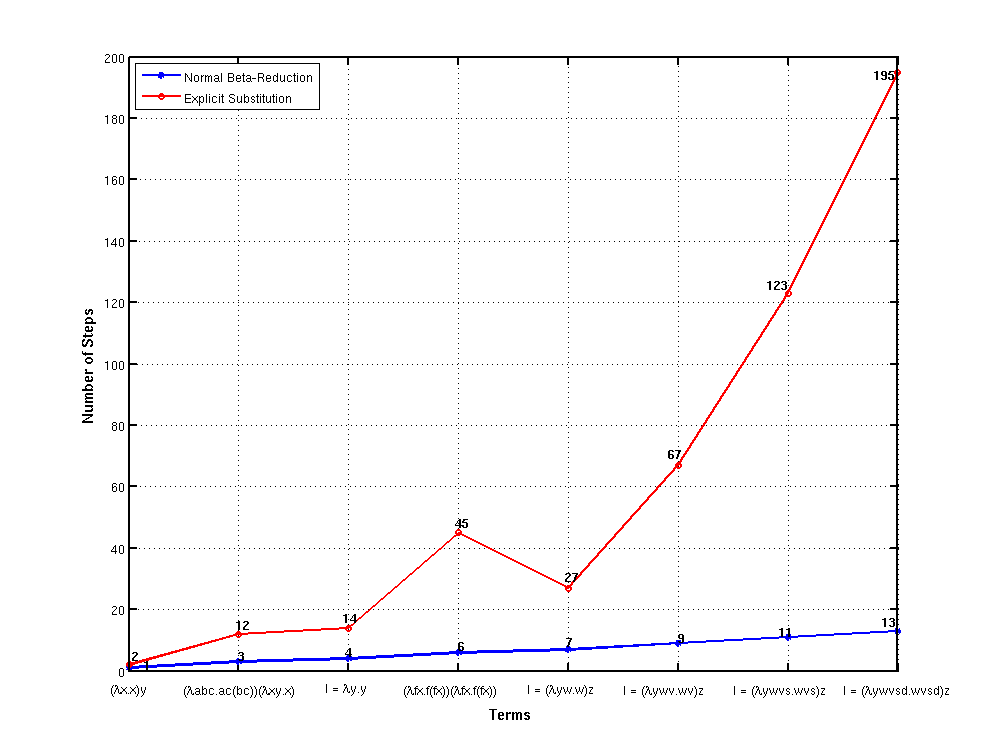
\includegraphics[width=\textwidth]{pics/zhang_01}
\caption{Reduction steps needed for normal $\beta$-reduction and explicit substitution}
\label{fig:betax}
\end{figure}

The figure \ref{fig:betax} illustrates the difference in the number of steps needed between normal $\beta$-reduction and $\xrightarrow[bx]{}$. As the term $I$ grows larger, the number of steps in normal $\beta$-reduction grows linearly, while xgc grows approximately exponentially. We can see that the $\beta$-reduction steps needed for term $(\lambda fx.f(fx))(\lambda fx.f(fx))$ is less than the steps needed when $I = (\lambda yw.w)z$, however, the number of explicit substitution steps is larger. The number of reduction steps mainly depends on the free occurrences of bound variables in an abstraction. For the term $(\lambda fx.f(fx))$, the free occurrence of $f$ and $x$ in $f(fx)$ lead to repeated substitution and increase the number of reduction steps.  


\subsection{$\xrightarrow[\beta ]{}$ vs $\xrightarrow[bx]{}$ vs $\xrightarrow[bxgc]{}$}

The explicit garbage collection simplifies several proofs. For the $\lambda$xgc-term $(xy)\langle z:=M\rangle$, since there is no free occurrence of $z$ in the term $xy$, so the substitution $\langle z:=M\rangle$ can be removed. Then it no longer needs to be pushed into the application $xy$ which costs more explicit substitution steps. The following table and chart would show the number of steps decreased, or in other words, the efficiency improved by garbage collection.  

\begin{table}[h!]
\centering
\begin{tabular}{|c|c|c|c|}\hline
$\lambda$-term & Normal Reduction & Explicit Substitution & bxgc\\ \hline
$(\lambda x.x)y$ & 1 & 2 & 2\\ \hline
$(\lambda abc.ac(bc))(\lambda xy.x)$ & 3 & 12 & 12\\ \hline
$I = \lambda y.y$ & 4 & 14 & 12\\ \hline
$(\lambda fx.f(fx))(\lambda fx.f(fx))$ & 6 & 45 & 45\\ \hline
$I = (\lambda yw.w)z$ & 7 & 27 & 18\\ \hline
$I = (\lambda ywv.wv)z$ & 9 & 67 & 35\\ \hline
$I = (\lambda ywvs.wvs)z$ & 11 & 123 & 58\\ \hline
$I = (\lambda ywvsd.wvsd)z$ & 13 & 195 & 87\\ \hline
\end{tabular}
\caption{Reduction steps needed for normal reduction, explicit substitution, and bxgc}
\label{tb:diffff}
\end{table}

Compared with Table \ref{tb:diff}, Table \ref{tb:diffff} lists additional the number of steps needed by explicit substitution and garbage collection. As we can see, there is no garbage collection performed for the term $(\lambda x.x)y$ and $(\lambda abc.ac(bc))(\lambda xy.x)$. When $I = \lambda y.y$, the garbage collection takes place at the 2nd and 6th reduction step when the term is \verb|\v.((\y.y)<x:=(\y.y)v>)(((\y.y)x)<x:=(\y.y)v>)| and \verb|\v.((\y.y)<x:=(\y.y)v>)(x<x:=(\y.y)v>)|. There is no occurrence of $x$ in \verb|\y.y| in both cases. So the substitution is the garbage and is removed. Therefore, the substitution would no be pushed into the abstraction and it reduces 2 reduction steps.

For the term $(\lambda fx.f(fx))(\lambda fx.f(fx))$, there is no garbage collection performed because of the repeated occurrence of $f$ and $x$. When the term $I$ is gradually enlarged, the number of steps reduced by garbage collection becomes larger. It decreases more than a half when $I = (\lambda ywv.wv)z$. The more the number of reduction steps needed by explicit substitution, the more steps reduced by garbage collection. We can see the difference in Figure \ref{fig:betaxgc}
  
\begin{figure}[h!]
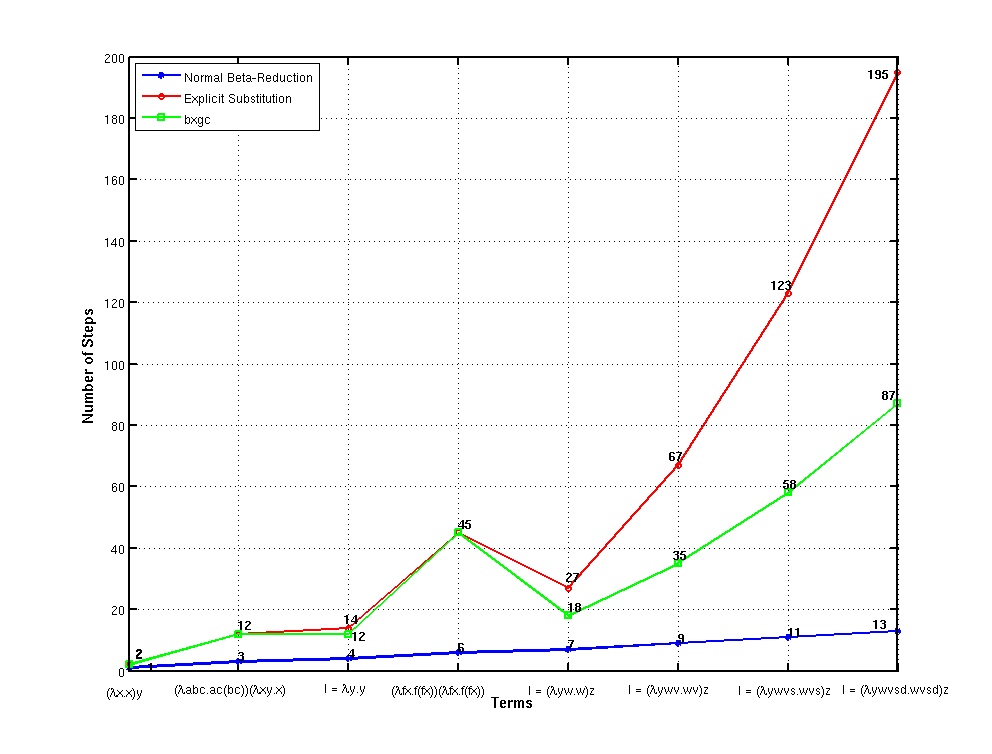
\includegraphics[width=\textwidth]{pics/zhang_02}
\caption{Reduction steps needed for normal reduction, bx, and bxgc}
\label{fig:betaxgc}
\end{figure}


The figure \ref{fig:betaxgc} illustrates the difference in the number of steps needed among normal $\beta$-reduction, $\xrightarrow[bx]{}$, and $\xrightarrow[bxgc]{}$. There is not too much difference between $\xrightarrow[bx]{}$ and $\xrightarrow[bxgc]{}$ for the first 4 terms. The garbage collection has a significant impact as the term $I$ grows larger. As we can see from the graph, the difference between $\xrightarrow[bx]{}$ and $\xrightarrow[bxgc]{}$ becomes larger from $I = (\lambda yw.w)z$ to $I = (\lambda ywvsd.wvsd)z$.

Although the garbage collection can remove any useless substitutions from $\lambda$xgc-terms and avoid redundant explicit substitution steps. It takes much more reduction steps than normal $\beta$-reduction. The number of steps needed by explicit substitution and garbage collection is approximately $nlogn$(only rough estimated).

It is worth mentioning that the reduction path of a term by different reduction strategies also affects the number of reduction steps needed for $\xrightarrow[bx]{}$ and $\xrightarrow[bxgc]{}$. The shortest $\xrightarrow[bxgc]{}$ path of the term $I = \lambda y.y$ is 8, using applicative order reduction. It costs 12 steps for the normal order reduction whereas all the $\beta$-reduction paths of it consist of 4 steps.  



